\documentclass[24pt,t,table, aspectratio=169]{beamer}

\usetheme[progressbar=frametitle]{metropolis}
\usepackage{appendixnumberbeamer}

\usepackage{booktabs}
\usepackage[scale=2]{ccicons}
\newcommand{\themename}{\textbf{\textsc{metropolis}}\xspace}

\setbeamercolor{background canvas}{bg=white}
\usepackage{framed}
\usepackage{mdframed}
\usepackage{siunitx}
\usepackage{hyperref}
\usetikzlibrary{decorations.pathmorphing}
\def\spiral#1{%
  \pgfmathparse{int(#1)}%
  \ifnum\pgfmathresult>0
    %\draw [help lines] (0,0) rectangle ++(1,1);
    \begin{scope}[shift={(1,1)}, rotate=90, scale=1/1.6180339887]
      \spiral{#1-1}
    \end{scope}
    \draw (0,0) arc (270:360:1);
  \fi
}


\newcommand{\atom}[3]{%
  \begin{scope}[shift={(#1,#2)}]
    % Proton (blue dot at center)
    \fill[blue] (0,0) circle (0.1) node[below left=2pt] {$p^+$};

    % Orbit path
    \draw[dashed,gray] (0,0) circle (0.6);

    % Electron (red dot on orbit)
    \fill[red] ({.6*cos(#3)},{.6*sin(#3)}) circle (0.1)
      node[above right=2pt] {$e^-$};
  \end{scope}%
}

\begin{document}

\begin{frame}[c, noframenumbering, plain]
  %\maketitle
  
  \large
  \begin{center}
  \begin{mdframed}[linecolor=orange, backgroundcolor=orange!20]
  \Large
  \centering
  \textbf{A Hybridized Discontinuous Galerkin Solver for Inductively Coupled Plasma}
  
  \small
  
  Nicolas Corthouts
  \end{mdframed}
  %\vspace{0.2cm}
  %\textcolor{orange}{\hrule}
  \end{center}
  \begin{center}
  \begin{tikzpicture}
  \draw (0,0) node{\includegraphics[width=.9\linewidth]{./cover_cropped.png}};
  \draw (0,-2.05) node{\reflectbox{\includegraphics[width = .9\linewidth, angle=180, origin=c]{./cover_cropped.png}}};
  \end{tikzpicture}
  \end{center}
  
%  \begin{minipage}[c]{.49\linewidth}
%  \small
%  \begin{tabular}{ll}
%  \textbf{Author} & Nicolas Corthouts\\ 
%  \textbf{Promoters} & Koen Hillewaert\\
%   & Thierry Magin
%  \end{tabular}
%  \end{minipage}
%  \begin{minipage}[c]{.49\linewidth}
%  \begin{tabular}{ll}
%  \textbf{Jury} & Christophe Geuzaine\\
%   & Peter Schütz \\
%   & Trevor Lafleur
%  \end{tabular}
%  \end{minipage}
%
%  \vspace{0.3cm}
  \includegraphics[height =1 cm]{2560px-University_of_Liège_logo.png}\hfill
\includegraphics[height=1 cm]{FRS-FNRS_ros_vert_transp.png}\hfill
\includegraphics[height =1 cm]{vki_logo_blue_rectangular.jpg}
  \vfill
\end{frame}

\section{Introduction}

\begin{frame}{Etats de la matière: eau à pression atmosphérique}

\begin{center}
\begin{tabular}{ccc}
\onslide<2->{\textbf{Solide}} & \onslide<3->{\textbf{Liquide}} & \onslide<4->{\textbf{Gaz}}\\
\onslide<2->{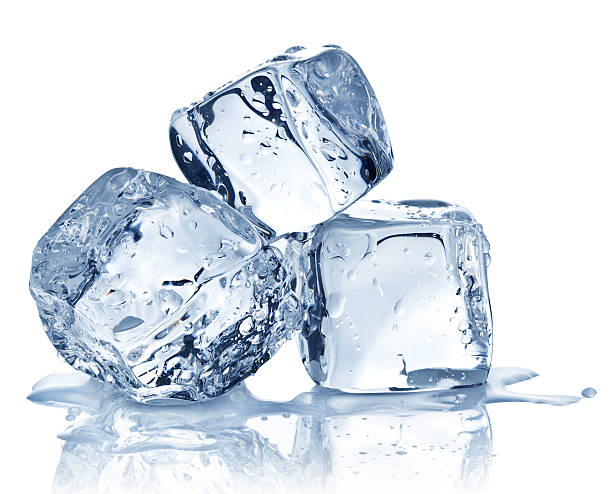
\includegraphics[height=.17\linewidth]{ice_cubes.jpg}} & \onslide<3->{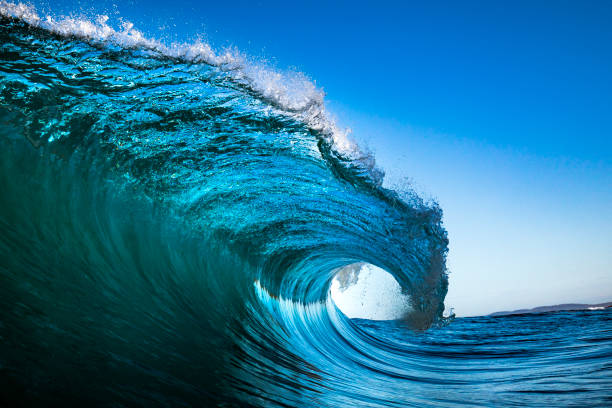
\includegraphics[height=.17\linewidth]{eau_liquide.jpg}} & \onslide<4->{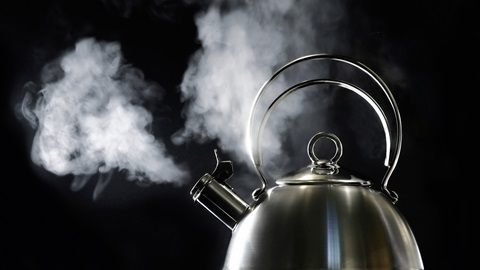
\includegraphics[height=.17\linewidth]{bouilloire.jpg}}\\
\onslide<2->{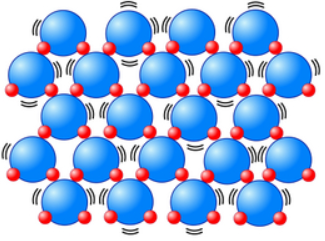
\includegraphics[height=.17\linewidth]{eau_solide.png}} & \onslide<3->{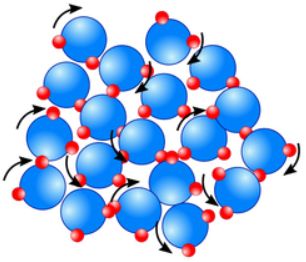
\includegraphics[height=.17\linewidth]{eau_liquide.png}} & \onslide<4->{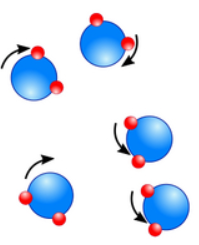
\includegraphics[height=.17\linewidth]{eau_gaz.png}}%\footnote{\tiny\url{https://www.assistancescolaire.com/eleve/3e/physique-chimie/reviser-une-notion/les-\%20etatsde-la-matiere-et-les-changements-d-etat-3_pc_01/print?print=1&printSheet=1}}\\
%\onslide<3->{
%$T \leq \SI{0}{\celsius}$ & $T \geq \SI{0}{\celsius}$ & $T \geq \SI{100}{\celsius}$
%}
\end{tabular}
\end{center}

\onslide<5>
{
\begin{framed}
\centering
\textbf{Que se passe-t-il si on chauffe encore plus?}
\end{framed}
}
\end{frame}

\begin{frame}{Translation, rotation et vibration}

\begin{center}
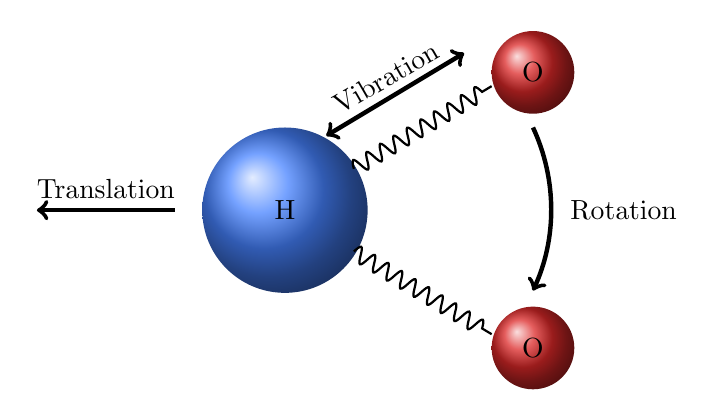
\begin{tikzpicture}[scale=3.5, spring/.style={decorate,decoration={coil,aspect=0,segment length=2mm,amplitude=1mm}}]

  % Oxygen atom color (blue)
  \definecolor{OxyBlue}{RGB}{70,130,255} % light-medium blue
  % Hydrogen atom color (red)
  \definecolor{HydRed}{RGB}{220,40,40}   % bright red

  % Oxygen atom
  \shade[ball color=OxyBlue] (0,0) circle (0.3);

  % Hydrogen atoms (approx 104° apart)
  \shade[ball color=HydRed] (0.9,0.5) circle (0.15);
  \shade[ball color=HydRed] (0.9,-0.5) circle (0.15);
  
  \node at (0,0) {H};
  \node at (0.9,0.5) {O};
  \node at (0.9,-0.5) {O};
  
  \draw[spring,thick] (0.25,0.15) -- (0.75,0.45);
  \draw[spring,thick] (0.25,-0.15) -- (0.75,-0.45);
  
  \onslide<2,5->{
  \draw[->, ultra thick] (-0.4,0) -- (-0.65,0) node[above]{Translation} -- (-0.9,0);
  }
  
  \onslide<3,5->{
  \draw[->,thick, ultra thick] (0.9,0.3) arc[start angle=25,end angle=-25,radius=.7];
  \node at (1., 0) [right]{Rotation};
  %\draw[bend right, ->, ultra thick] (0.9,-0.5) -- (0.9,0.5);
  }
  
  \onslide<4,5->{
  \draw[<->,thick, ultra thick] (0.15,0.27) -- (0.65,0.57);
  \node at (0.4, .42) [above, rotate=30] {Vibration};
  %\draw[bend right, ->, ultra thick] (0.9,-0.5) -- (0.9,0.5);
  }

  % Optional arrows to mimic rotation (as in your image)
  %\draw[->,thick] (0.35,0.55) arc[start angle=100,end angle=20,radius=0.6];
  %\draw[->,thick] (0.35,-0.55) arc[start angle=-100,end angle=-20,radius=0.6];

\end{tikzpicture}
\end{center}

%Les molécules vibrent, tournent et se déplacent de plus en plus vite. Les electrons sont excités jusqu'à ce que certains se détachent et se meuvent librement.
\end{frame}

\begin{frame}{Excitation et ionization}

\begin{center}
\begin{tikzpicture}[scale=3.5, spring/.style={decorate,decoration={coil,aspect=0,segment length=2mm,amplitude=1mm}}]

  % Oxygen atom color (blue)
  \definecolor{OxyBlue}{RGB}{70,130,255} % light-medium blue
  % Hydrogen atom color (red)
  \definecolor{HydRed}{RGB}{220,40,40}   % bright red

  % Oxygen atom
  \shade[ball color=OxyBlue] (0,0) circle (0.3);
  
  \node at (0,0) {H};
 
  \onslide<2->
  {
  	\def\dist{1.5}
  	\fill[blue] (\dist,0) circle (0.03) node[below left=2pt] {$p^+$};

  	% Orbit path (optional, dashed)
  	\draw[dashed,gray] (\dist,0) circle (.5);

	\draw[->, ultra thick] (.4, 0) -- (.9,0);

  	% Electron (red dot on orbit)
  	\def\ang{40} % position angle
  }
  
  \onslide<2>{
  	\fill[red] ({\dist+.5*cos(\ang)},{.5*sin(\ang)}) circle (0.03) 
  	node[below left] {$e^-$};
  }
  
  \onslide<3->
  {
  	\fill[red!50] ({\dist+.5*cos(\ang)},{.5*sin(\ang)}) circle (0.03) 
  	node[below left] {$e^-$};
  }  
  
  \onslide<3>
  {
  	\draw[dashed,gray] (\dist,0) circle (.7);
  	\fill[red] ({\dist+.7*cos(\ang)},{.7*sin(\ang)}) circle (0.03) 
  	node[above right] {$e^-$};
  	\draw[->, ultra thick, red] ({\dist+.55*cos(\ang)},{.55*sin(\ang)}) -- ({\dist+.65*cos(\ang)},{.65*sin(\ang)});
  }
  
  
  \onslide<4>
  {
  	%\draw[dashed,gray] (\dist,0) circle (.9);
  	\fill[red] ({\dist+.9*cos(\ang)},{.9*sin(\ang)}) circle (0.03) 
  	node[above right] {$e^-$};
  	\draw[->, ultra thick, red] ({\dist+.9*cos(\ang)+0.1},{.9*sin(\ang)}) -- ({\dist+.9*cos(\ang)+0.1+0.5},{.9*sin(\ang)});
  }

\end{tikzpicture}

\only<3>
{
	\begin{framed}
	\centering
	Si l'énergie reçue le permet, l'électron est dans un état \textcolor{red}{\textbf{excité}}. Il reviendra à son état initial en émettant de la lumière: c'est la \textbf{\textcolor{red}{radiation}}.
	\end{framed}
}

\only<4>
{
	\begin{framed}
	\centering
	Si l'énergie reçue est trop grande, l'électron est arraché: il devient \textcolor{red}{\textbf{libre}}. L'atome d'hydrogène a été \textbf{\textcolor{red}{ionisé}}.
	\end{framed}
}

\end{center}

\end{frame}

\begin{frame}{Plasma: le quatrième état de la matière}
\centering
\begin{tabular}{cc}
\begin{tikzpicture}
\node at (0,0) {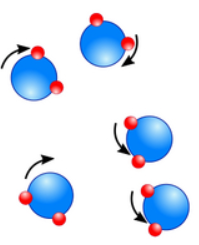
\includegraphics[height=.3\linewidth]{eau_gaz.png}};
\end{tikzpicture}
&
\onslide<2->
{
\begin{tikzpicture}
\node at (0,0) {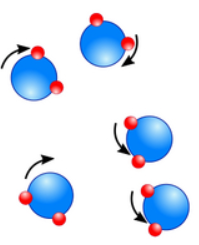
\includegraphics[height=.3\linewidth]{eau_gaz.png}};
\fill[red] (0,0) circle (0.1) node[above right] {$e^-$};
\fill[red] (1,1) circle (0.1) node[above right] {$e^-$};
\fill[red] (-1,-0.3) circle (0.1) node[above right] {$e^-$};
\node[blue] at (-1.7,.7) {\textbf{+}};
\node[blue] at (1.4,0) {\textbf{+}};
\end{tikzpicture}
}\\
\textbf{Gaz neutre} & \onslide<2->{\textbf{Plasma}}
\end{tabular}

\only<3>{
\begin{framed}
\textbf{Un plasma est un gaz quasi-neutre composé de particules chargées (ions $\textcolor{blue}{\bullet^+}$ et electrons $\textcolor{red}{\bullet^{e^-}}$) et neutres ($\bullet^n$) démontrant un comportement collectif.\footnotemark}
%A plasma is a quasi-neutral gas of charged and neutral particles which exhibits collective behaviour.
\end{framed}
}
\only<3>{\footnotetext[1]{\tiny F. F. Chen. Introduction to Plasma Physics and Controlled Fusion. Ed. by Springer International Publisher. 2016}}

\end{frame}

\begin{frame}{Comportement collectif du plasma}
\centering
\begin{framed}
\textbf{Collision = interaction entre particules}
\end{framed}

\begin{tabular}{cc}
\onslide<2->{\textbf{Collisions de courte portée}} & \onslide<3->{\textbf{Collisions de longue portée}}\\
\onslide<2->{
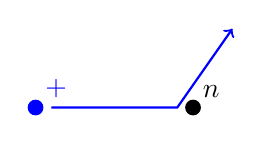
\begin{tikzpicture}
\fill[blue] (0,0) circle (0.1) node[above right] {$+$};
\fill[black] (2,0) circle (0.1) node[above right]{$n$};
\draw[blue, ->, thick] (0.2,0) -- (1.8, 0) -- (2.5, 1);
\end{tikzpicture}} &
\onslide<3->{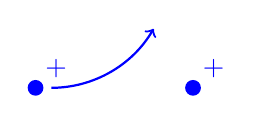
\begin{tikzpicture}
\fill[blue] (0,0) circle (0.1) node[above right] {$+$};
\fill[blue] (2,0) circle (0.1) node[above right] {$+$};
\draw[->,blue, thick] (0.2,0) arc[start angle=-90,end angle=-30,radius=1.5];
\end{tikzpicture}}\\
\onslide<2->{Contact direct (local \& binaire)} & \onslide<3->{Force électrique (à distance, collectif)}
\end{tabular}
\onslide<4->{
\begin{framed}
Si l'échelle est suffisamment grande ($> \SI{1}{\micro\meter}$ dans notre cas), le plasma est \textbf{\textcolor{red}{quasi-neutre}} grâce à la force électrique.
\end{framed}
}
\end{frame}

\begin{frame}{Plasma dans la vie de tous les jours}

\begin{framed}
\centering
\textbf{Les plasmas composent 90\% de l'univers visible.}
\end{framed}
\begin{center}
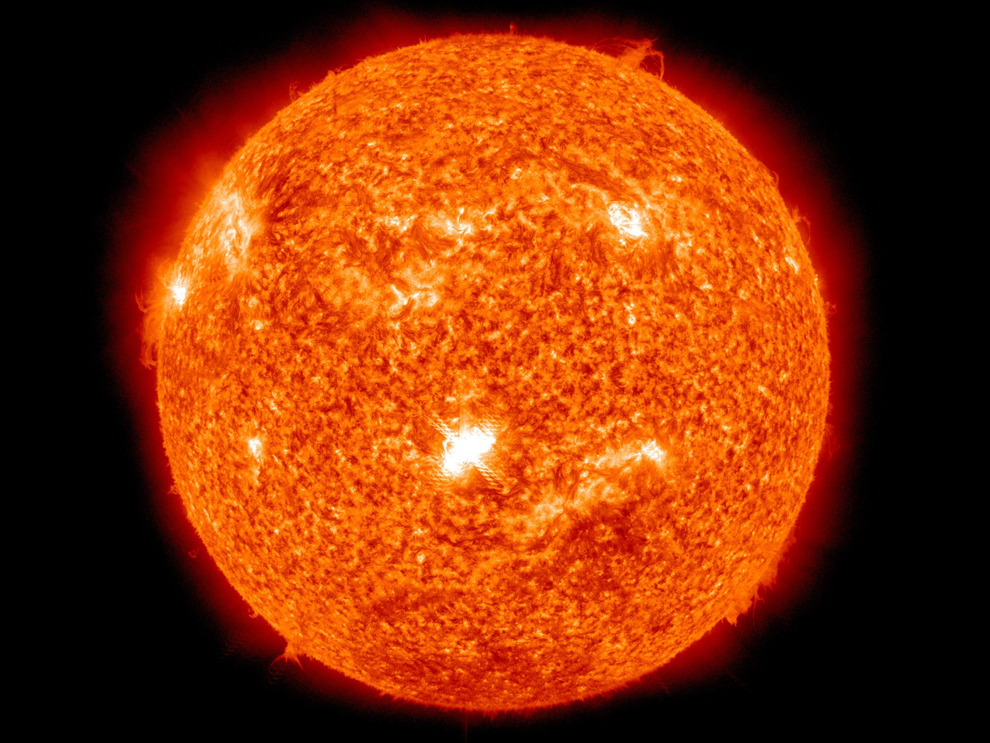
\includegraphics[height=.22\linewidth]{./sun.jpg}
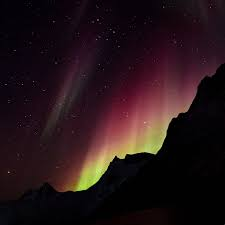
\includegraphics[height=.22\linewidth]{./aurora_borealis.jpeg}
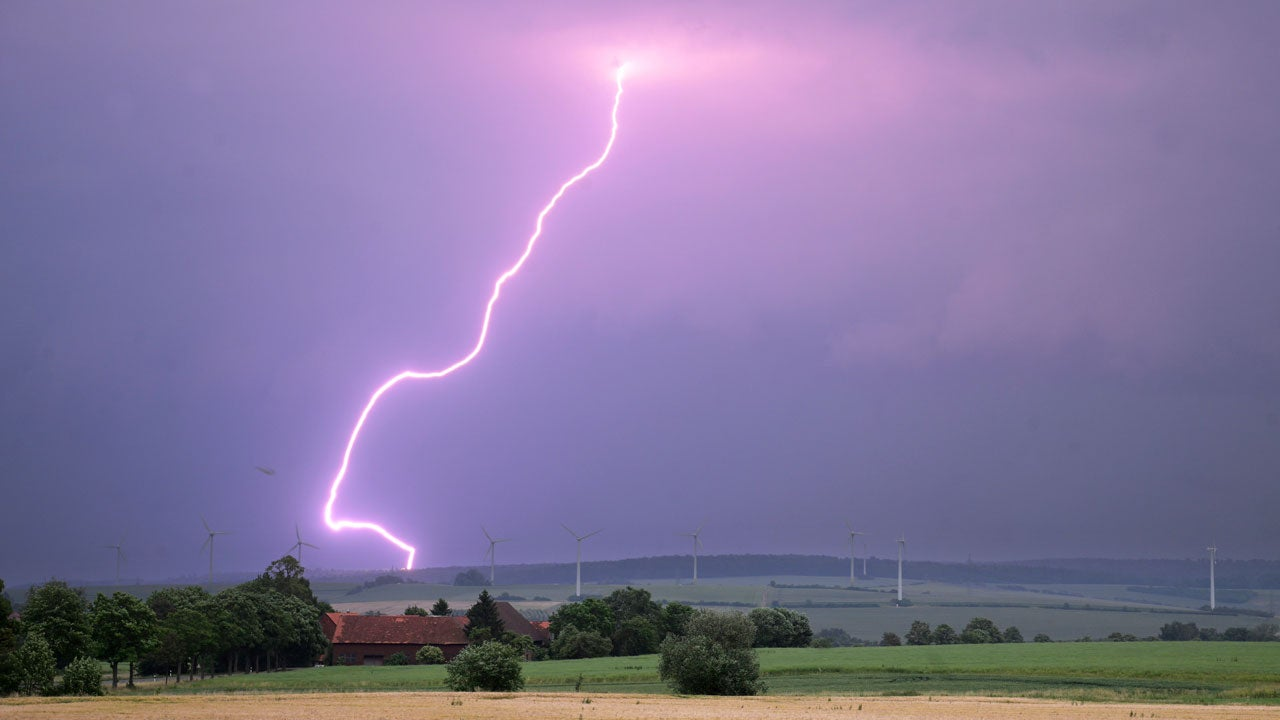
\includegraphics[height=.22\linewidth]{./lightning.jpg}
\end{center}
De plus en plus d'applications: fusion nucléaire, médecine, métallurgie, lasers, création de microprocesseurs, ...
\end{frame}

\begin{frame}{Plasma froids}

\begin{framed}
\textbf{Pour les plasma froids, l'énergie est d'abord emmagasinée par les éléctrons libres et cédée lors des collisions aux ions lourds.}
\end{framed}
En fonction de l'efficacité des collisions, deux scénarii sont possibles:
\begin{center}
\begin{tabular}{cc}
\textbf{Collisions peu efficaces} & \textbf{Collisions efficaces}\\
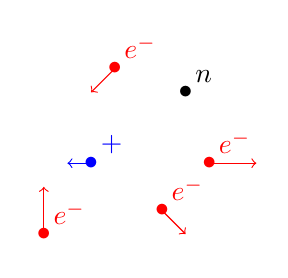
\begin{tikzpicture}[scale=3]
\node[blue] at (0,0) {$\bullet$};
\node at (.4,.3) {$\bullet$};
\node[red] at (.5,0) {$\bullet$};
\node[red] at (.3,-.2) {$\bullet$};
\node[red] at (-.2,-.3) {$\bullet$};
\node[red] at (.1,.4) {$\bullet$};
\draw[red, ->] (.5,0.) -- (.7, 0.);
\draw[red, ->] (.3,-.2) -- (.4, -.3);
\draw[red, ->] (-.2,-.3) -- (-.2, -.1);
\draw[red, ->] (.1,.4) -- (0., .3);
\draw[blue, ->] (0,0) -- (-0.1,0);
\node[blue] at (0,0) [above right]{$+$};
\node at (.4,.3) [above right]{$n$};
\node[red] at (.5,0) [above right]{$e^-$};
\node[red] at (.3,-.2) [above right]{$e^-$};
\node[red] at (-.2,-.3) [above right]{$e^-$};
\node[red] at (.1,.4) [above right]{$e^-$};
\end{tikzpicture}
 &
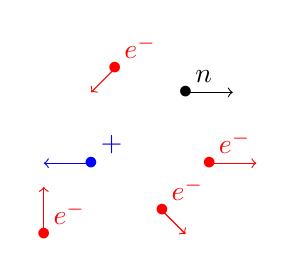
\begin{tikzpicture}[scale=3]
\node[blue] at (0,0) {$\bullet$};
\node at (.4,.3) {$\bullet$};
\node[red] at (.5,0) {$\bullet$};
\node[red] at (.3,-.2) {$\bullet$};
\node[red] at (-.2,-.3) {$\bullet$};
\node[red] at (.1,.4) {$\bullet$};
\draw[red, ->] (.5,0.) -- (.7, 0.);
\draw[red, ->] (.3,-.2) -- (.4, -.3);
\draw[red, ->] (-.2,-.3) -- (-.2, -.1);
\draw[red, ->] (.1,.4) -- (0., .3);
\draw[blue, ->] (0,0) -- (-0.2,0);
\draw[->] (.4,.3) -- (.6,.3);
\node[blue] at (0,0) [above right]{$+$};
\node at (.4,.3) [above right]{$n$};
\node[red] at (.5,0) [above right]{$e^-$};
\node[red] at (.3,-.2) [above right]{$e^-$};
\node[red] at (-.2,-.3) [above right]{$e^-$};
\node[red] at (.1,.4) [above right]{$e^-$};
\end{tikzpicture}\\
$T_e \gg T_h$ & $T_e \simeq T_h$
\end{tabular}
\end{center}


\end{frame}

\begin{frame}{Plasma en réentrée atmosphérique}
\centering
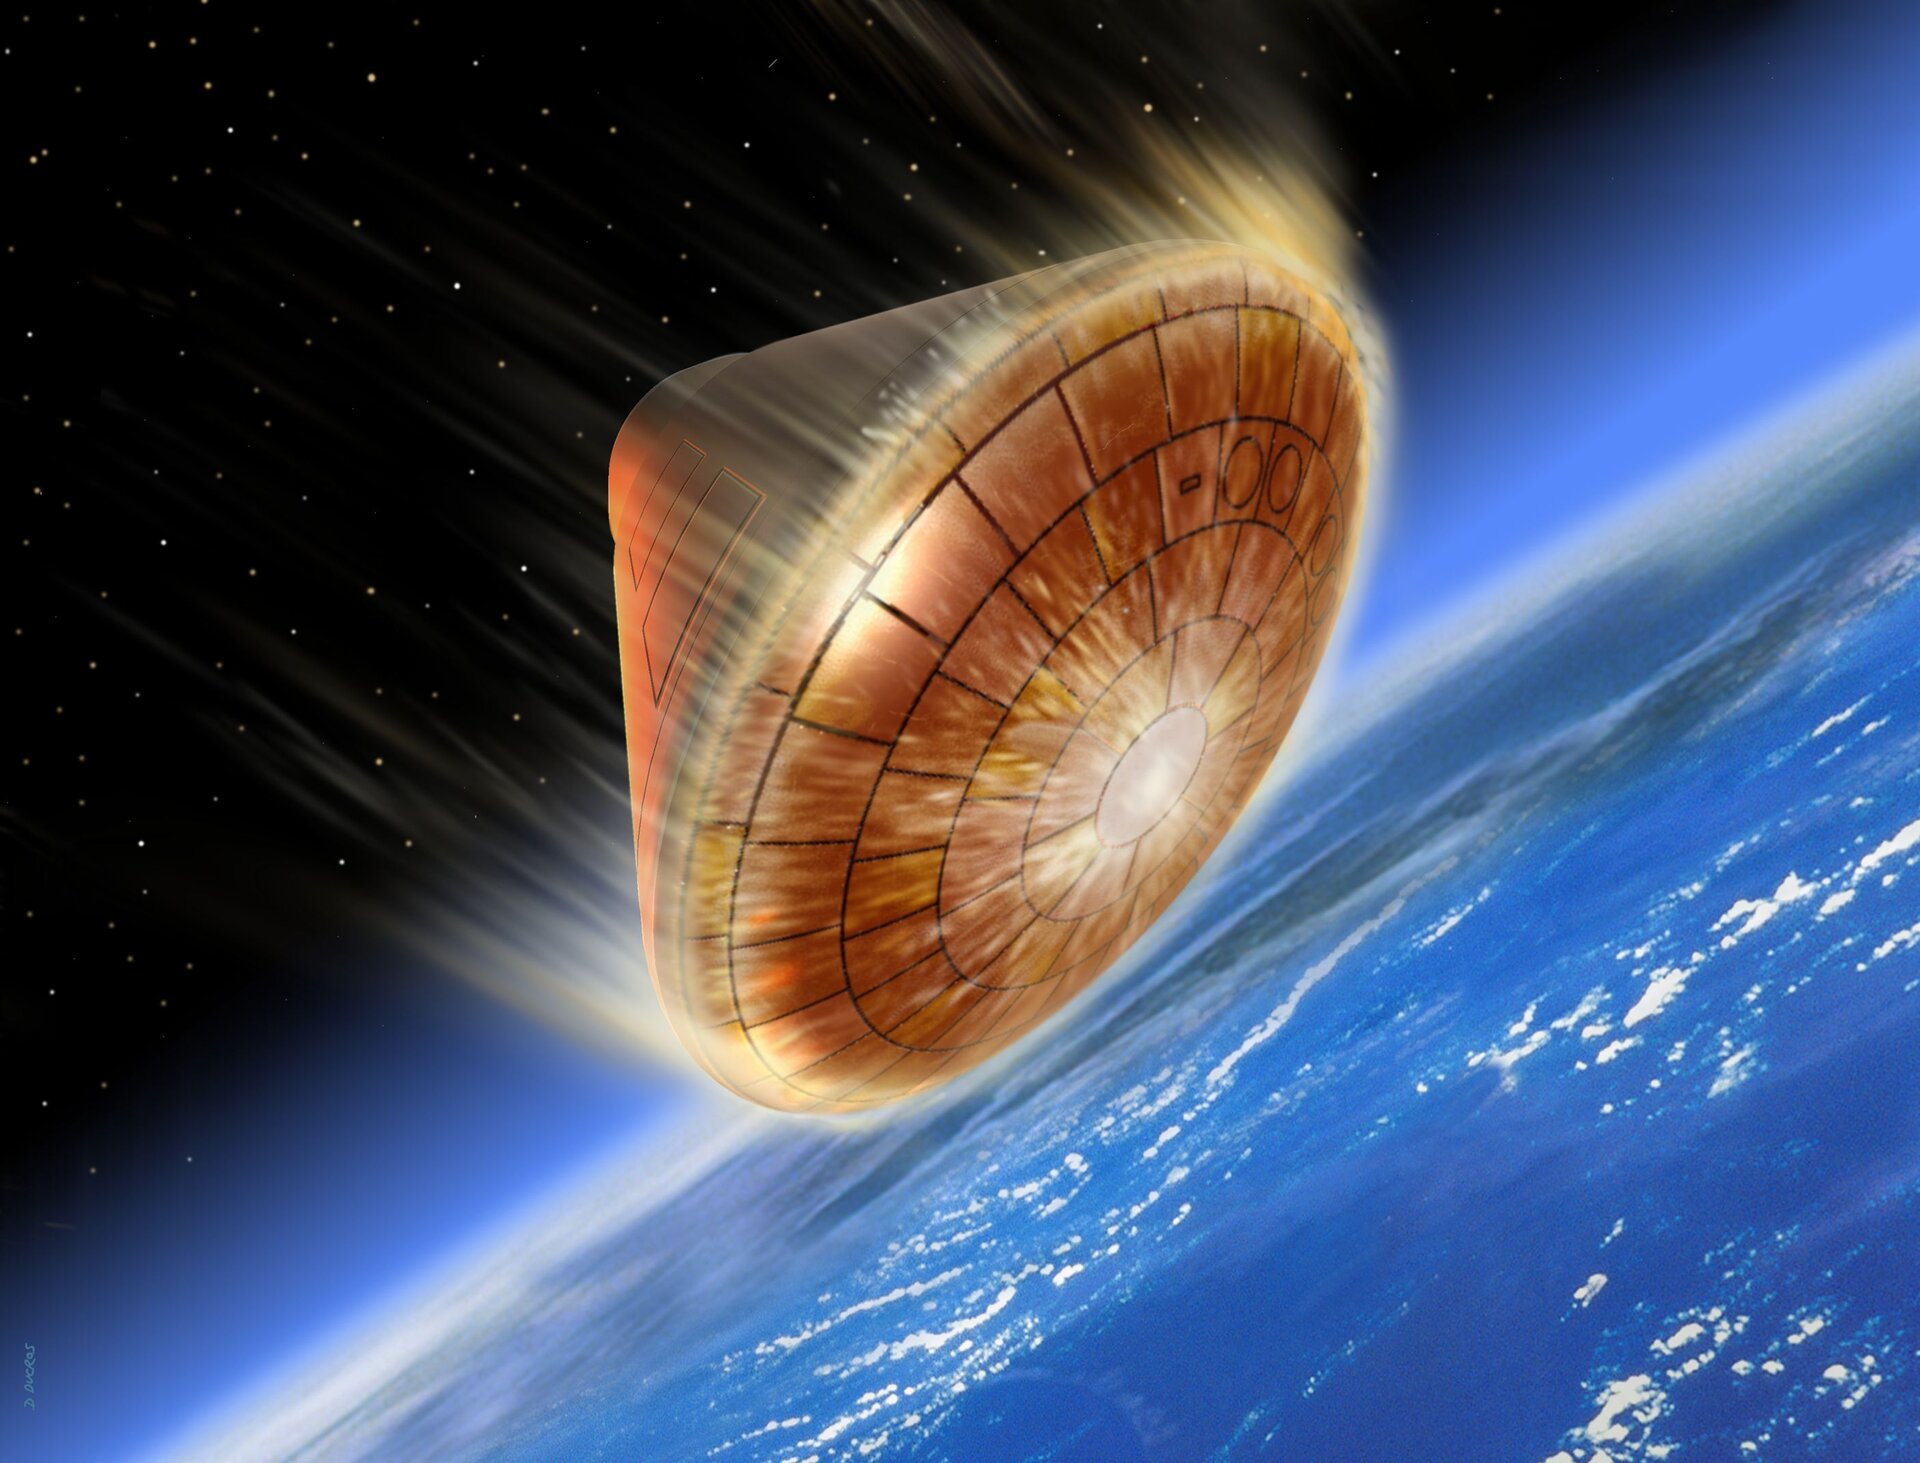
\includegraphics[height=.35\linewidth]{./reentry_esa.jpg}
\begin{framed}
La grande vitesse de réentrée $\simeq\SI{10}{\kilo\meter\;\second^{-1}}$, un choc suffisamment fort pour ioniser l'air $\Rightarrow$ plasma.
\end{framed}
\end{frame}

\begin{frame}{Sytème de protection thermique et destruction des déchets spatiaux}
\centering
\begin{tabular}{cc}
\onslide<2->{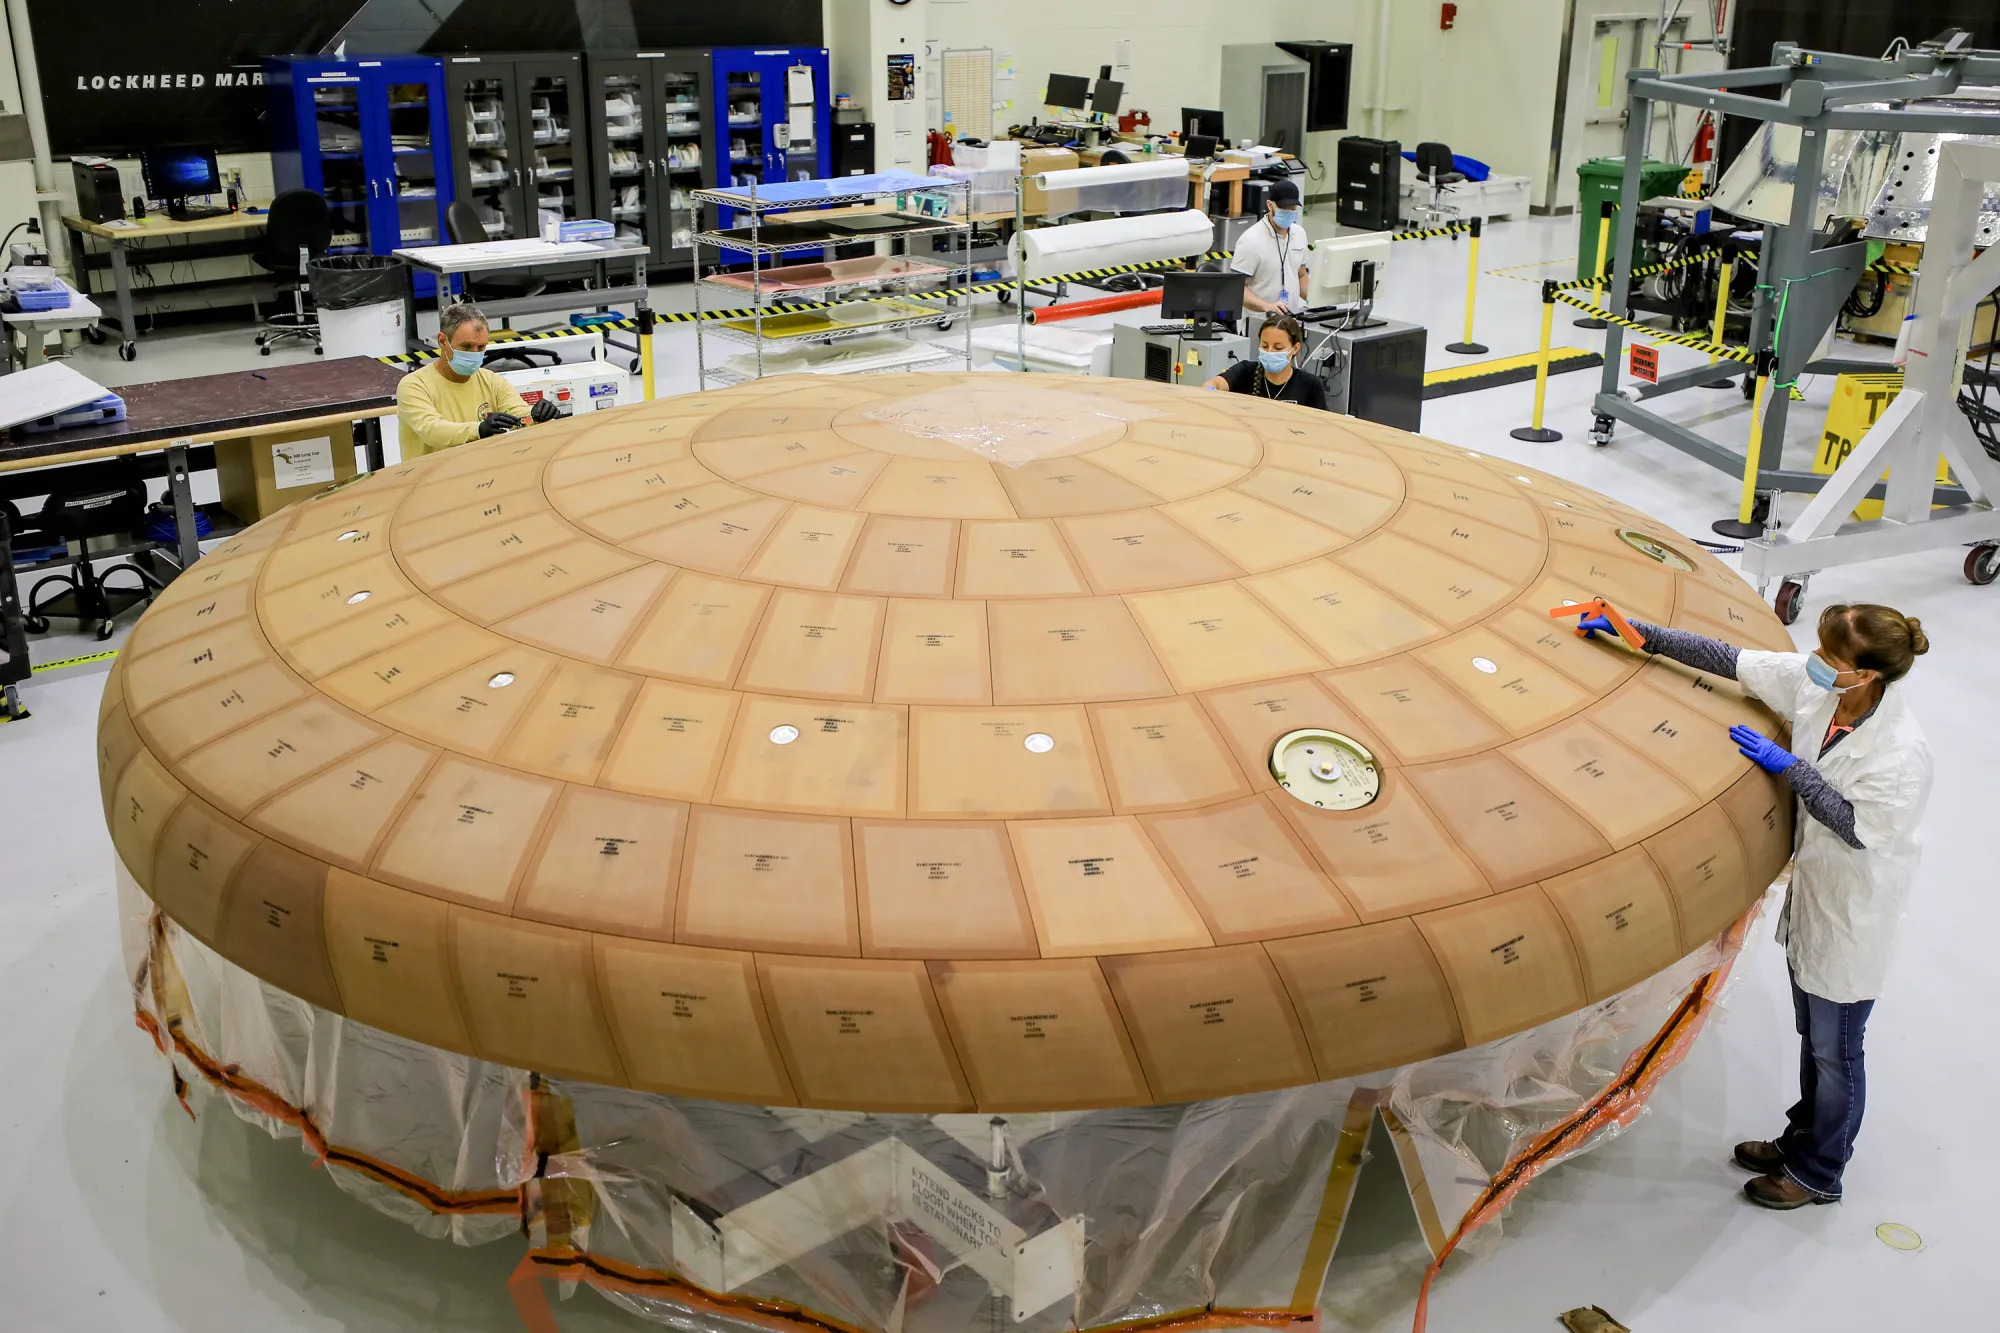
\includegraphics[height=.3\linewidth]{./heat_shield.jpg}} &
\onslide<3->{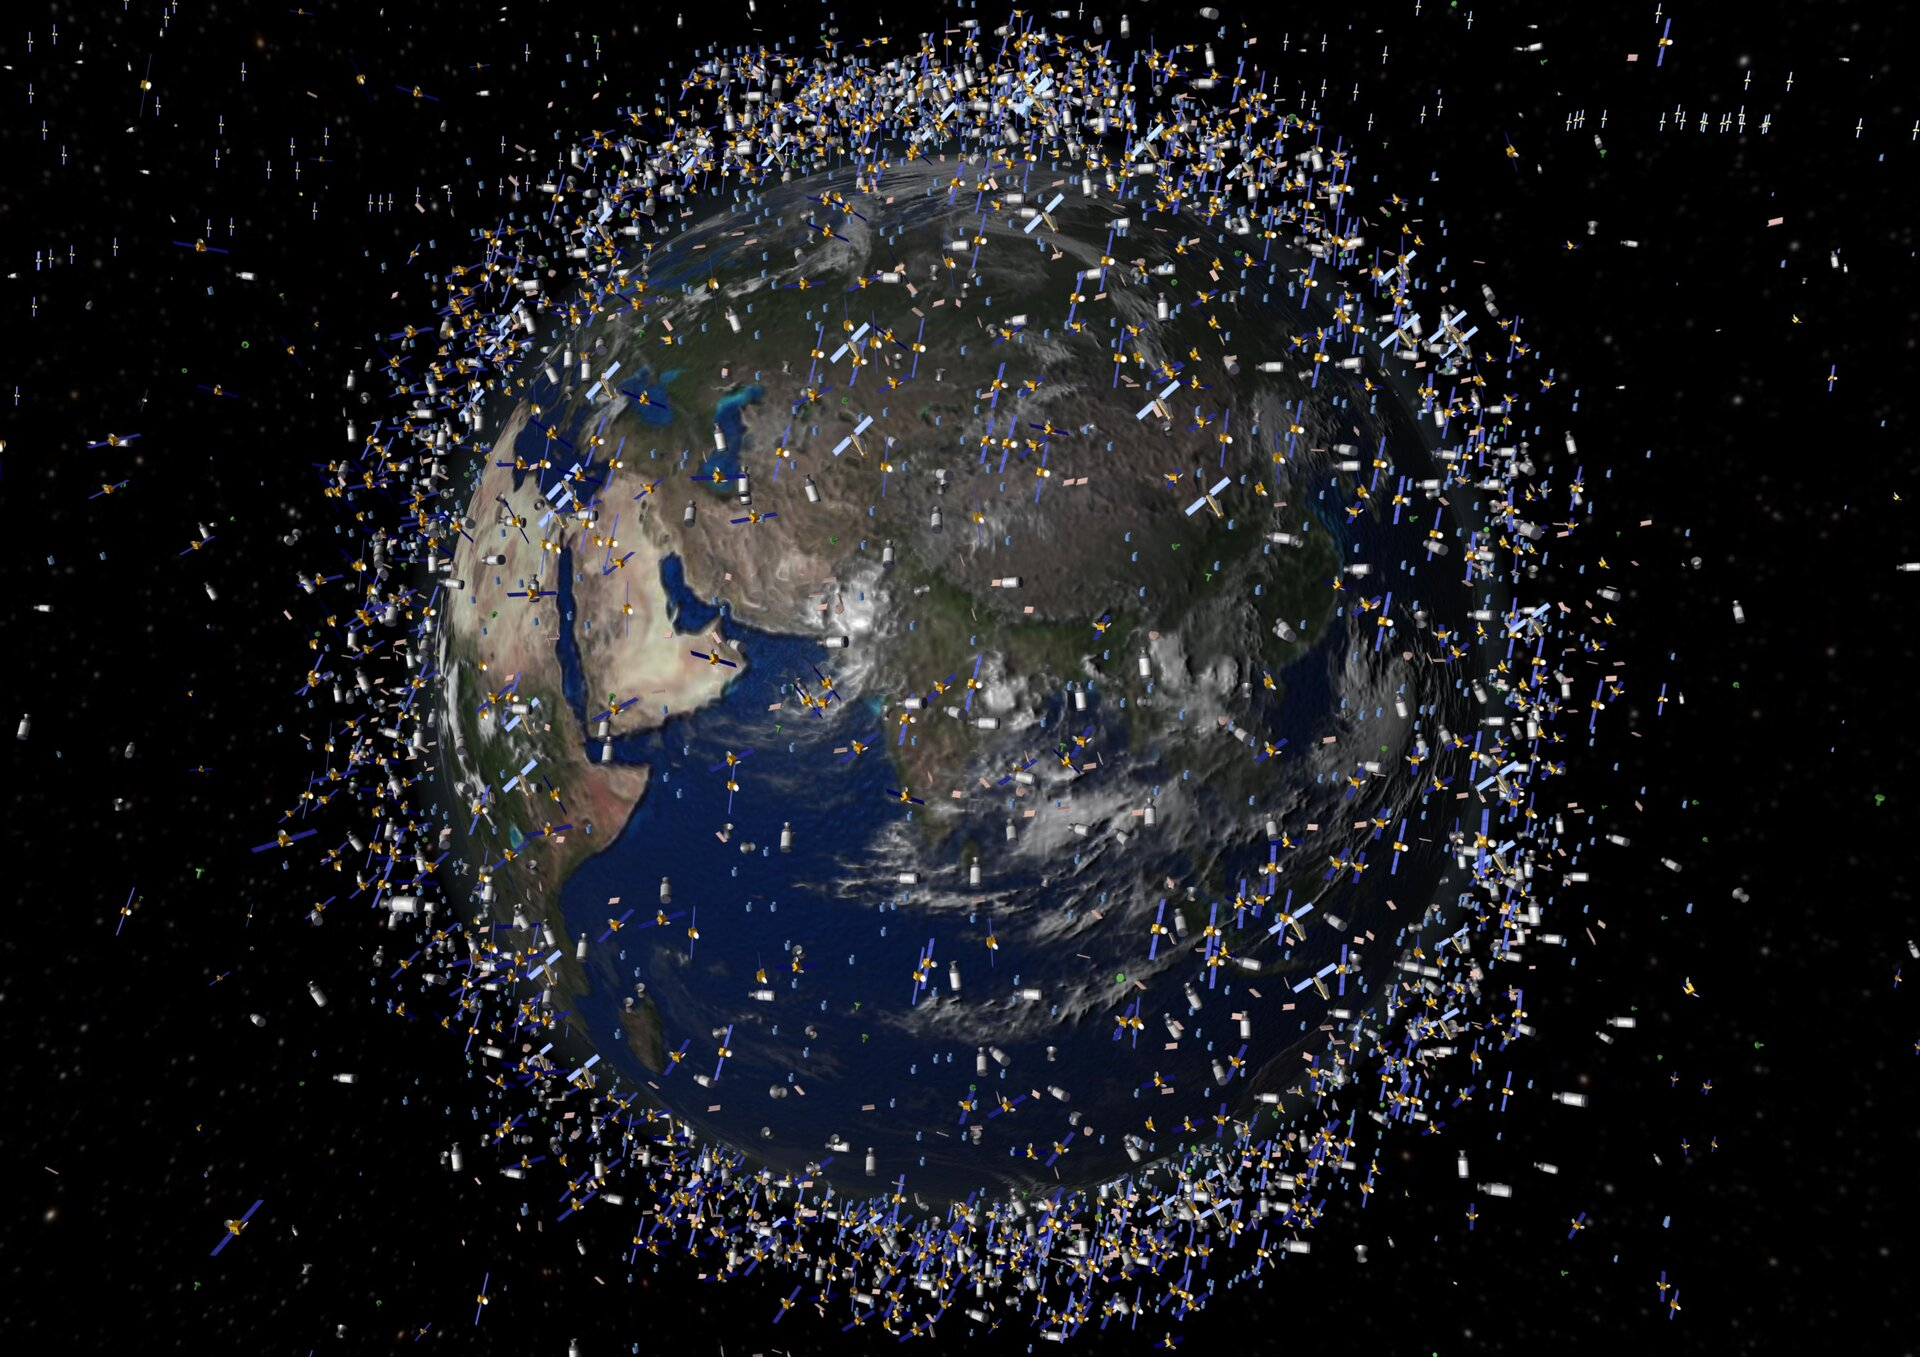
\includegraphics[height=.3\linewidth]{./vizualisation_satellites_esa.jpg}}\\
\onslide<2->{\textbf{TPS}} & \onslide<3->{\textbf{Déchets spatiaux}}
\end{tabular}
\onslide<4->{
\begin{framed}
\textbf{Nécessité de développer des machines expérimentales reproduisant les plasmas de réentrée atmosphérique pour étudier ces applications.}
\end{framed}
}
\end{frame}

\begin{frame}{Plasma à induction}
\begin{minipage}[t]{0.5\linewidth}
    \centering
    \vspace{0.7cm}
    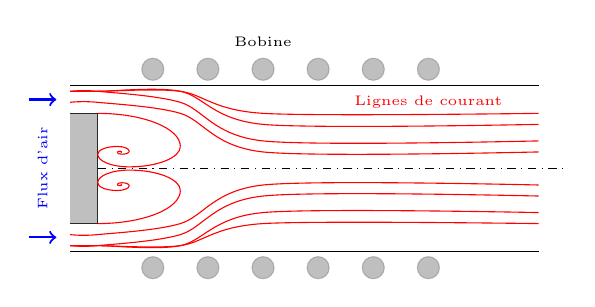
\begin{tikzpicture}[scale=0.7]
      \draw[dash dot] (0,0) -- (8.5,0);
      \draw[-] (-0.5,-1) -- (0, -1) -- (0,1) -- (-0.5,1);
      \fill[gray, opacity=0.5] (-0.5,-1) -- (0, -1) -- (0,1) -- (-0.5,1) -- (-0.5,-1);
      \draw[-] (-0.5,1.5) -- (8,1.5);
      \draw[-] (-0.5,-1.5) -- (8,-1.5);
      \foreach \x in {1,2,...,6}{
        \filldraw[gray, opacity = 0.5] (\x, 1.8) circle (0.2);
        \filldraw[gray, opacity = 0.5] (\x, -1.8) circle (0.2);
      }
      \begin{scope}[red]
      \begin{scope}[yshift=1cm,yscale=-0.6,xscale=1.5]
      \spiral{10}
      \end{scope}
      \begin{scope}[yshift=-1cm,yscale=0.6,xscale=1.5]
      \spiral{10}
      \end{scope}
      \draw plot [help lines, smooth] coordinates {(-0.5,1.2) (0,1.2) (1.5, 1.0) (3, 0.3) (8, 0.3)};
      \draw plot [help lines, smooth] coordinates {(-0.5, -1.2) (0,-1.2) (1.5, -1.0) (3, -0.3) (8, -0.3)};
      
      \draw plot [help lines, smooth] coordinates {(-0.5, 1.4) (0,1.4) (1.5, 1.2) (3, 0.5) (8, 0.5)};
      \draw plot [help lines, smooth] coordinates {(-0.5, -1.4) (0,-1.4) (1.5, -1.2) (3, -0.5) (8, -0.5)};
      
      \draw plot [help lines, smooth] coordinates {(-0.5, 1.4) (0, 1.4) (1.5, 1.4) (3, 0.8) (8, 0.8)};
      \draw plot [help lines, smooth] coordinates {(-0.5, -1.4) (0, -1.4) (1.5, -1.4) (3, -0.8) (8, -0.8)};
      
      \draw plot [help lines, smooth] coordinates {(-0.5, 1.4) (0, 1.4) (1.5, 1.4) (3, 1.0) (8, 1.0)};
      \draw plot [help lines, smooth] coordinates {(-0.5, -1.4) (0, -1.4) (1.5, -1.4) (3, -1.0) (8, -1.0)};
      
      \draw (6,1.2) node{\tiny \textcolor{red}{Lignes de courant}};
      \draw (3,2.3) node{\tiny \textcolor{black}{Bobine}};
      \draw (-1,0) node{\tiny \rotatebox{90}{\textcolor{blue}{Flux d'air}}};
      \end{scope}
      
      %\draw (2,0.2) node{$T\simeq \SI{}{10^4\kelvin}$};
      \draw[blue, ->, thick](-1.25, 1.25) -- (-0.75,1.25);
      \draw[blue, ->, thick](-1.25, -1.25) -- (-0.75,-1.25);
      %\draw (3.5,2.3) node{\includegraphics[width=0.1\linewidth]{AC_Sign.png}};
      %\draw (6,1.2) node{$p \simeq \SI{}{10^4\pascal}$};
      
    \end{tikzpicture}
    
    \vspace{0.45cm}
    Torche
    \end{minipage}
    \begin{minipage}[t]{0.49\linewidth}
    \centering
    \vspace{0.5cm}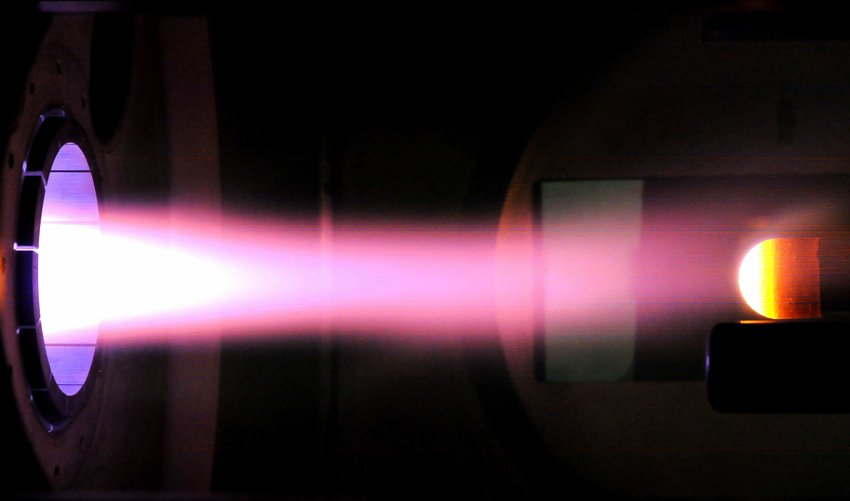
\includegraphics[width=\linewidth]{Ablation-testing-at-the-Plasmatron-ICP-facility-of-the-VKI-3.jpg}
    
    Chambre
    \end{minipage}
    
    \only<1>
    {
    Examples: Plasmatron (VKI), Plasmatron X (Illinois), IPG (Russie), ...
    
    Basé sur le principe de \textbf{transfer de chaleur local}.
    }
    \only<2>
    {
    	Equation de Maxwell, Navier-Stokes + modèles physico-chimiques.
    }
    %Physique de l'électromagnétisme, equations de la mécanique des fluides, et chimie/thermodynamique.
\end{frame}

\begin{frame}{Plasma à induction: besoin de plus}

\begin{center}
\begin{framed}
\textbf{Des solvers numériques ont été développés afin de préparer au mieux les expériences dans les torches à induction.}
\end{framed}
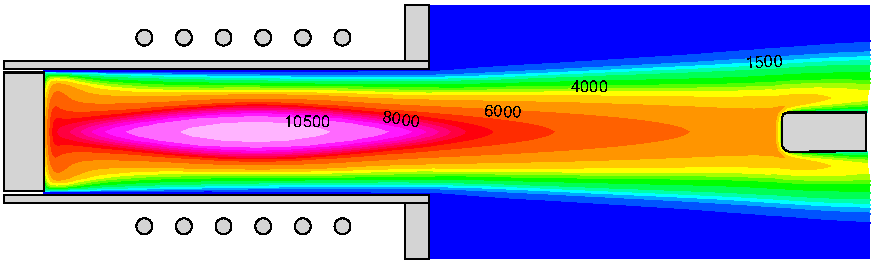
\includegraphics[width=.7\linewidth]{lhtsT.pdf}\footnote{\tiny Thierry Magin.}
\end{center}
\end{frame}

\begin{frame}{Solver actuels}
\begin{framed}
La plupart des solvers actuels permettent de représenter des écoulements axisymmétriques en régime établi et avec un modèle chimique et thermique simple.
\end{framed}

Il faut pouvoir aussi représenter...

\centering
\begin{tabular}{cc}
\onslide<2->{
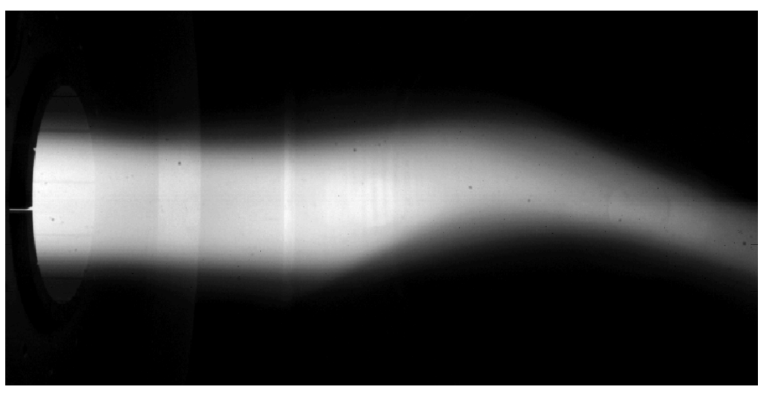
\includegraphics[height=.25\linewidth]{./plasma_jet_unsteady_experimental.png}}
& \onslide<3->{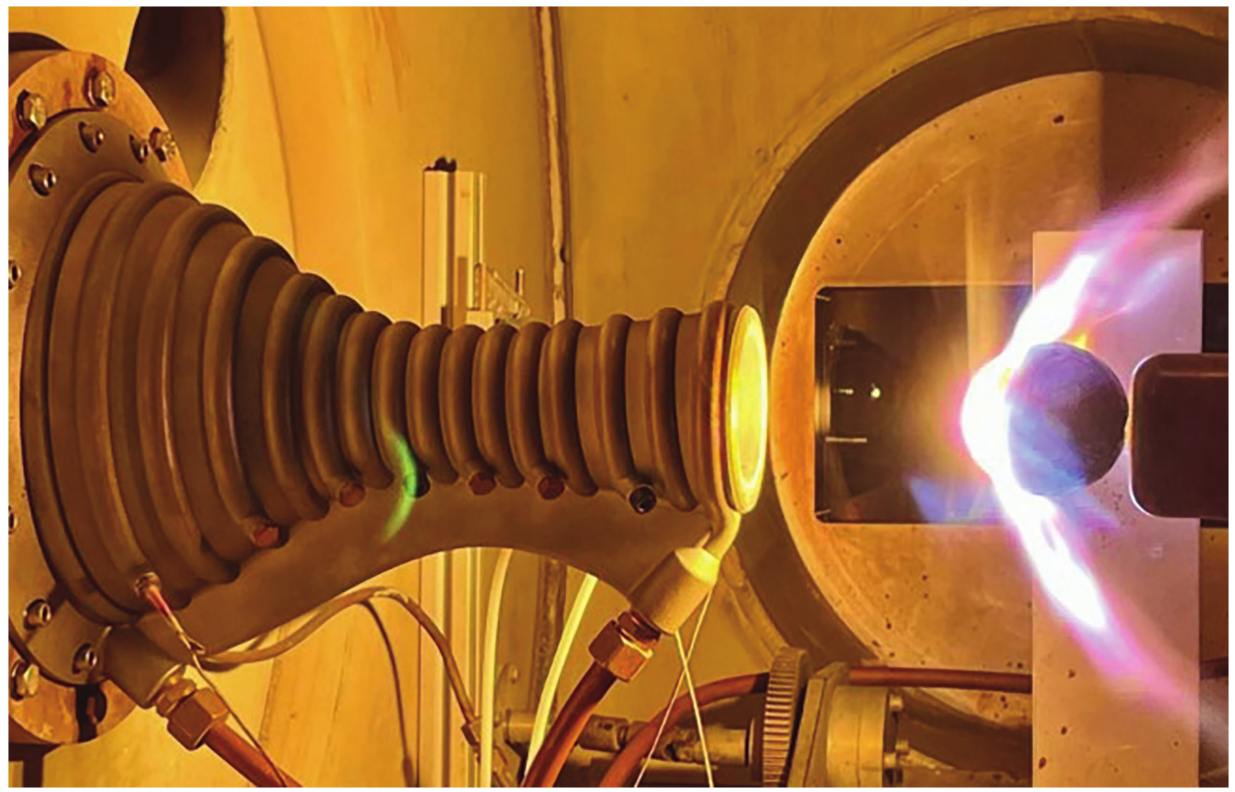
\includegraphics[height = .25 \linewidth]{./plasmatron_nozzle_operating.png}} \\
\onslide<2->{Instationnarités} & \onslide<3->{Effets 3D et géométries complexes} 
\end{tabular}

\end{frame}



\end{document}